\subsubsection{Модель самоорганизации экситонов с переносом заряда}\label{subsubsec:antonyuk}
\nomenclature{ЭПЗ}{Экситоны с переносом заряда}

В основе модели, предложенной Б.~П.~Антонюком и В.~Б.~Антонюком~\cite{antonyuk2001self} лежит представление о возникновении в германосиликатном стекле нового типа возбуждений --- экситонов с переносом заряда (ЭПЗ). При облучении волокна зелёным светом с длиной волны $\lambda = 532$~нм электрон покидает примесный Ge-центр и переходит в матрицу или на другой Ge-центр, образуя пространственно разделённую пару электрон--дырка.

Согласно экспериментальным данным по спектрам поглощения и люминесценции (в том числе наведённым УФ-облучением), ЭПЗ обладает полосой поглощения шириной $\Delta_{\text{ЭПЗ}}\sim 0.1$~эВ с максимумом при энергии порядка $\varepsilon_{ЭПЗ}=2.22$~эВ, что соответствует длине волны $560$~нм.

При наложении постоянного электрического поля $E_0$ уровни ЭПЗ расщепляются, как показано на рис.~\ref{fig:epz_spectra}. Состояние с большей энергией соответствует дипольному моменту, направленному против поля, а состояние с меньшей энергией~--- дипольному моменту, направленному по полю. Поскольку частота накачки больше частоты, соответствующей максимуму поглощения в отсутствие постоянного поля, расщепление приводит к тому, что высокоэнергетическое состояние оказывается более вероятным, чем низкоэнергетическое. Следовательно, большинство ЭПЗ ориентируется дипольным моментом против поля. Поляризация создаёт поле, сонаправленное с исходным. Таким образом, возникает положительная обратная связь: поле способствует преимущественному возбуждению ЭПЗ, дипольный момент которых направлен против поля, что приводит к усилению поля.

\nomenclature[N]{$\varepsilon_{\text{ЭПЗ}}$~[\si{\electronvolt}]}{Энергия максимума полосы поглощения ЭПЗ, $\varepsilon_{\text{ЭПЗ}} = 2.22$~эВ ($\lambda = 560$~нм)}

\nomenclature[N]{$E_0$~[\si{\volt\per\meter}]}{Комплексная амплитуда квазистатического электрического поля, индуцированного в процессе оптического полинга}
\nomenclature[N]{$d_{\text{ЭПЗ}}$~[\si{\coulomb\meter}]}{Дипольный момент экситона с переносом заряда (ЭПЗ)}
\nomenclature[N]{$\Delta_{\text{ЭПЗ}}$~[\si{\electronvolt}]}{Ширина полосы поглощения ЭПЗ, $\Delta_{\text{ЭПЗ}} \approx 0.1$~эВ}
\nomenclature[N]{$E_{0,\text{sat}}$~[\si{\volt\per\meter}]}{Напряжённость статического поля в состоянии насыщения, $E_{0,\text{sat}} \sim 10^5$~В/см}
\nomenclature[N]{$q_e$~[\si{\coulomb}]}{Элементарный заряд}
\nomenclature[N]{$r_{\text{ЭПЗ}}$~[\si{\meter}]}{Характерный размер ЭПЗ (расстояние между электроном и дыркой), $r_{\text{ЭПЗ}} \sim 10$~Å}

Насыщение поля $E_0$ наступает, когда расщепление $d_{\text{ЭПЗ}}E_0$ становится сравнимым с шириной полосы $\Delta_{\text{ЭПЗ}}\approx0.1$~эВ. При этом $E_{\text{0, sat}} \sim \Delta_{\text{ЭПЗ}}/d_{\text{ЭПЗ}}=\Delta_{\text{ЭПЗ}}/(q_e  r_{\text{ЭПЗ}})\sim 10^5$~В/см.
%, что согласуется с прямыми измерениями~\cite{dominic1994high}.
Здесь $q_{e}$~---заряд электрона,  $r_{\text{ЭПЗ}}\sim10~\si{\angstrom}$~---характерный размер ЭПЗ.


\begin{figure}[h]
	\centering
	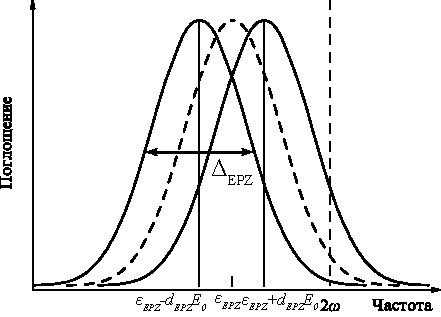
\includegraphics[width=0.6\linewidth]{Dissertation/images/review/epz_spectra}
	\caption{Расщепление полосы поглощения ЭПЗ во внешнем поле $E_0$. При $2\omega > \varepsilon_{\text{ЭПЗ}}$ преимущественно возбуждаются ЭПЗ с дипольным моментом $\mathbf{d}_{\text{ЭПЗ}}$, направленным против $\mathbf{E_0}$}
	\label{fig:epz_spectra}
\end{figure}

%Эксперимент, позволивший разделить два механизма, был проведён в 1992 году \cite{djanov1992photo}. Советский и российский учёный Евгений Дианов c коллегами предложили методику, основанную на существенной роли границы освещаемой области: при изменении граничного заряда в рамках зарядовой модели распределение электрического поля изменится значительно, а в рамках ориентационной~--- слабо. Из-за этого при смещении освещаемой области вдоль направления разделения зарядов представляется возможным создать протяжённую область заряда одного знака и малую~--- другого. При этом будут наблюдаться три максимума электрического поля (рис. \ref{fig:expsplit}, слева) и, как следствие, три максимума эффективности генерации гармоники. При движении в перпендикулярном направлении, равно как при работе в рамках ориентационной модели, зарядовые области будут одного размера и область эффективной генерации также будет однородной. Эксперимент подтвердил предположения авторов (рис. \ref{fig:expsplit}, справа)), и зарядовые модели стали доминирующими среди прочих предлагаемых физических механизмов генерации второй гармоники в оптическом волокне.
%
%\begin{figure}
%	\centering
%	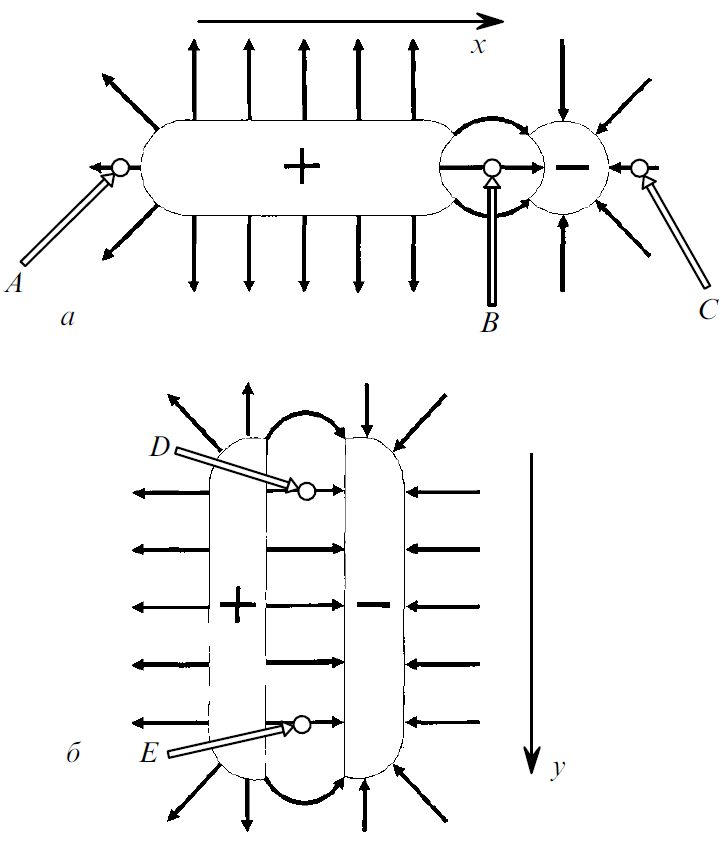
\includegraphics[width=0.5\linewidth]{Dissertation/images/review/expSplit.jpg}
%	\caption{Слева: распределение электрического поля в зарядовой модели при движении пятна света параллельно (а) и перпендикулярно (б) направлению разделения зарядов. Справа: мощность второй гармоники при движении в соответствующих направлениях}
%	\label{fig:expsplit}
%\end{figure}
%
%
%На основании проведённой работы коллектив Диановского волоконного центра предложил и развил зарядовую модель, основанную на анизотропном когерентном фотовольтаическом эффекте \cite{dianov1995photoinduced}.
%
%
%%Как отмечалось в главе про волокно, для достижения волноводного эффекта в световодах посредством увеличения показателя преломления сердцевины волокна необходимо добавлять в плавленый кварц соответствующие примеси. Именно они и являются источником дефектов, приводящих в конечном счёте к фотоиндуцированной генерации второй гармоники.
%%

%В 2000 году была предложена физическая модель, объединяющая зарядовые и ориентационные особенности предыдущих моделей \cite{antonyuk2001self}. Проводя анализ спектров комбинационного, гиперкомбинационного и люминесцентного спектра оптического волокна, легированного оксидом германия, авторы предложили модель усиления слабого затравочного поля, основанную на самоорганизации возбуждений в среде. Согласно этой модели, примесный электрон, находящийся на Ge-центре поглощает один квант волны второй гармоники (зелёный свет) и переходит либо на другой Ge-центр, либо в силикатную матрицу.  Создаётся \textsf{экситон с переносом заряда (ЭПЗ)}, представляющий собой электрический диполь. Рассматривая электрон-дырочную кинетику в среде, авторы пришли к выводу, что экситоны с переносом заряда представляют собой систему с обратной положительной связью и ориентируются в слабом постоянном электрическом поле так, чтобы его усилить до величины $E\approx10^5~\text{В}/\text{см}$.
%%
%Далее авторы объединяют свою модель с уже существующими, рассматривая усиление слабой волны второй гармоники в периодическом (по длине) электрическом поле, созданным экситонами с переносом заряда. Учёт истощения накачки приводит к первому в мире правильному объяснению временной зависимости эффективности генерации, а также резкому увеличению мощности с последующим спадом при изменении фазовых соотношений между волнами накачки и второй гармоники.
%
%Представим изложенную логику генерации второй гармоники в виде схемы:
%\begin{figure}[h]
%	\centering
%	\includegraphics[width=0.99\linewidth]{Dissertation/images/review/scheme_ЭПЗ}
%	\caption{Упрощённая схема физических процессов при генерации второй гармоник в волокне согласно \cite{antonyuk2001self}}
%	\label{fig:schemeЭПЗ}
%\end{figure}
%Как следует из схемы, изображённой на рис. \ref{fig:schemeЭПЗ}, в предложенной автором модели находят отражение первые теоретические объяснения эффекта, изложенные сразу после его экспериментального наблюдения.


